%!TEX root = proyecto.tex

\chapter{Diseño y resolución}

\linespread{1.5}

\section{Paul Viola and Michael Jones}

En 2001, el reconocimiento facial tuvo su primera apararicion en el campo de la visión artificial como aplicación en tiempo real. Este avance fue de la mano de Paul Viola y Michael Jones, expertos de la Universidad de Cambridge. Análogamente, el punto de partida del estudio de este TFG. Durante este apartado, se estudiará el funcionamiento del algoritmo ideado por estos dos investigadores y se realizará una implementación del mismo mediante \textit{Python} y \textit{OpenCV} para comprobar como se comporta en la situación actual.

\subsection*{Método de estudio}

El trabajo de los expertos fue presentado por parte de la Universidad de Cambridge mediante un \textit{paper} (ensayo de la investigación). Y se introduce como: 
\begin{quote}
	"This paper describes a machine learning approach for visual object detection which is capable of processing images extremely rapidly and achieving high detection rates" \cite{paulViola}
\end{quote}

Para poder lograr esta afirmación se basan en un procedimiento de trabajo en dos fases: entrenamiento y detección. Igualmente, Paul y Michael lo dividen en tres puntos importantes: una imagen integral, Adaboost (algoritmo de Machine Learning) y un método llamado \textit{cascade}. 

Con todos estos puntos combinados lograron ingeniar un prototipo capaz de detectar caras humanas con un \textit{frame rate} de 15 fps. Fue diseñado para la detección de caras frontales, haciendose difícil para posiciones laterales o inclinadas.

Las imagenes que se toman para realizar la detección pasan por una transformación del espacio de color a \textit{grayscale}. Con el objeto de encontrar caracteristicas en ellas, llamadas \textit{haar-like features}. Nombradas así por su inventor Alfred Haar en el siglo XIX. En este trabajo se hacen uso de tres tipos de haar-like features, que son las siguientes:

\begin{figure}[htp]
	\centering
	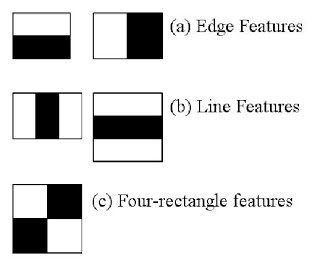
\includegraphics[width=5cm]{imagenes/haar-like.jpeg}
	\caption{Haar-like Features}
	\label{fig:haarLike}
\end{figure}

Las \textbf{\textit{Haar-like features}}, o también conocidas como \textit{Haar-wavelet} son una secuencia de funciones \textit{rescaled square-shaped}, siendo similares a las funciones de Fourier y con un comportamiento parecido a los \textit{Kernel} usados en las \textit{Redes Convolucionales} (matrices que consiguen extraer ciertas \textit{features} de la imagen de entrada). De manera que, las \textit{Haar Features} serán las características de la detección facial.

En un estudio ideal, los pixeles que forma el \textit{feature} tendra una division clara entre pixeles de color blanco con los de color negro (Figura 4.1), pero en la realidad eso casi nunca se va a dar.

Más especificamente, las \textit{Haar-like features} estan compuestas por valores escalares que representan la media de intensidades entre dos regiones rectangulares de la imagen. Estas capturan la intesidad del gradiente, la frecuencia espacial y las direcciones, mediante el cambio del tamaño, posición y forma de las regiones rectangulares basandose en la resolución que se define en el detector. \cite{haar-like}

Estas características van a ayudar al ordenador a entender lo que es la imagen estudiada. Van a ser utilizadas mediante \textit{Machine Learning} para detectar donde hay una cara o no, mediante un recorrido sobre toda la imagen. Esto conlleva una potencia de computación elevada. Para paliar este problema idearon el método de la \textit{Imagen Integral}.

La \textbf{\textit{Imagen Integral}} permite calcular sumatorios sobre subregiones de la imagen, de una forma casi instantanea. Además de ser muy útiles para las \textit{HAAR-like features}, tambien lo son en muchas otras aplicaciones.

Si se supone una imagen con unas dimensiones de $<w,h>$ (ancho y alto, respectivamente), la imagen integral que la representa tendrá unas dimensiones de $<w+1,h+1>$. La primera fila y columna de esta son ceros, mientras que el resto tendrán el valor de la suma de todos los pixeles que le preceden. \cite{integral-web} Ahora, para caluclar la suma de los pixeles en una region especifica de la imagen, se toma la correspondiente en la imagen integral y se suma según la siguiente fórmula (siguiendo la numeración de la Figura \ref{fig:integral}):
\begin{center}
	$sum = L4 + L1 - (L2 + L3)$ 
\end{center}
\begin{figure}[htp]
	\centering
	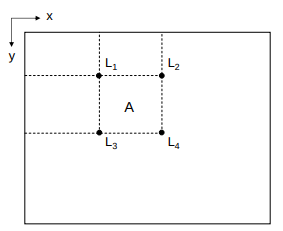
\includegraphics[width=5cm]{imagenes/integral.png}
	\caption{Imagen Integral}
	\label{fig:integral}
\end{figure}

Viola y Jones junta esta propuesta con los filtros \textit{Haar-like features}, y consiguen computar dichas características de manera constante y eficaz. \cite{integral}\\

% ---------------------------
%https://aishack.in/tutorials/integral-images-opencv/

%https://www.quora.com/How-integral-image-is-used-in-image-processing-and-how-improves-the-computation-time?share=1
%https://www.quora.com/What-are-the-must-read-papers-in-the-field-of-computer-vision-for-a-student-in-pursuing-research-in-the-field
% ---------------------------
%
% MACHINE LEARNING - ADABOOST
\newpage
Una vez estudiada la obtención de caracteristcas y con un set de entrenamiento, solo queda seleccionar un método de \textit{machine learning} que permita crear una función de clasificación. Concretamente, se plantea el uso de una variante de \textbf{\textit{AdaBoost}}. Este algoritmo de aprendizaje ...



% https://www.math.arizona.edu/~hzhang/math574m/Read/explaining-adaboost.pdf
%
%
% ---------------------------
%

% VIDEO DE LOCOS: https://www.youtube.com/watch?v=uEJ71VlUmMQ&t=5s

\subsection*{Implementación}

\subsection*{Experimentación}

\begin{itemize}
	\item Inicios del reconocimiento facial
	\item Explicar su funcionamiento
	\item Mostrar funcionamiento y aplicacion al objetivo
\end{itemize}



\section{HOG y Dlib}

\begin{itemize}
	\item Explicar su funcionamiento
	\item Mostrar funcionamiento y aplicacion al objetivo
\end{itemize}

\section{Facial Landmask}

\begin{itemize}
	\item Explicar su funcionamiento
	\item Mostrar funcionamiento y aplicacion al objetivo
\end{itemize}

\section{Facial Landmask Custom}

\begin{itemize}
	\item Plantear idea
	\item Proceso de creacion
	\item Mostrar funcionamiento y aplicacion al objetivo
\end{itemize}

\section{YOLO}

\begin{itemize}
	\item Acercamiento al Deep Learning
	\item Explicar su funcionamiento
	\item Mostrar funcionamiento y aplicacion al objetivo
\end{itemize}

\section{Tensorflow}

\begin{itemize}
	\item Plantear idea
	\item Procedimiento
	\item Mostrar funcionamiento y aplicacion al objetivo
\end{itemize}